\thispagestyle{plain}
\selectlanguage{spanish}
\begin{abstract}
Si bien el modelo estándar de partículas configura la teoría más completa de la composición de la materia y sus interacciones, hay preguntas y fenómenos que este no puede explicar como la materia y energía oscura, la gravedad cuántica, la masa de los neutrinos y la jerarquía de las interacciones. Con el fin de encontrar respuestas a diversos interrogantes en la física se han propuesto extensiones al modelo estándar de partículas, algunas de las cuales sugieren la existencia de bosones neutros masivos llamados bosones $Z'$. Esta investigación busca caracterizar la producción de bosones $Z'$ mediante dos mecanismos en particular. El primero es el mecanismo de Drell-Yan, que consiste en la aniquilación de un quark y un anti-quark produciendo un bosón $Z'$ que decae finalmente en un par leptón-antileptón. El segundo mecanismo se conoce como Vector Boson Fusion. En este mecanismo dos quarks intercambian bosones $W$ o $Z$, que se fusionan en un bosón masivo $Z'$. Para la caracterización de estos procesos se buscará construir la matriz de dispersión (matriz $S$) y a partir de ella se calcularán secciones transversales de producción. Hasta el momento se obtuvo el término de interacción de los bosones $Z'$ con fermiones. A partir de este término se podrá calcular las secciones eficaces de producción mediante el mecanismo Drell-Yan. Resta calcular el término de interacción con otro bosones para poder describir la producción mediante Vector Boson Fusion.
\end{abstract}


\section{Introduction}




The Standard Model (SM) of particle physics is the best theory so far to describe particles and their interactions \cite{zyla_review_2020}. However, the SM faces serious challenges; to name a few, the SM fails to explain neutrino masses \cite{mohapatra_neutrino_1980,Fukuda_1999,Ahmad_2002,Eguchi_2003}, gravity \cite{donoghue_effective_2012}, or the dark-matter content of the universe \cite{dodelson_sterile_1994}. These shortcomings hint towards new physics beyond the SM. 

The search for new physics is an ongoing effort, which often involves probing flavour processes and comparing experimental measurements with their SM predictions. Recent results show deviations from SM predictions in $B^+$ mesons decays. At the quark level, the anti-beauty quark, $\overline{b}$, in the $B$-meson decays into second-generation quarks and leptons according to $\overline{b}\rightarrow \overline{s}\ell^+ \ell^-$ and $\overline{b}\rightarrow \overline{c}\ell^+ \nu_\ell$. In the SM, such processes are mediated by virtual electroweak bosons ($\gamma$, $W^\pm$, $Z^0$). Under the SM, different leptons have the same interaction strengths, so the decay rates for $B^+ \rightarrow K^+\ell^+\ell^-$ across lepton generations should be identical. However, experimental data from proton-proton collisions show large deviation from theoretical values \cite{lhcbcollaboration2021test, lhcb_measurement}. Despite not reaching the threshold of statistical significance, these results point towards lepton flavour universality (LFU) violation. To account for these anomalies, several references have proposed the existence of a new hypothetical particle called the leptoquark \cite{alonso_lepton_2015,FAJFER2016270,ASSAD2018324,blanke_b_2018,barbieri_b-decay_2018,calibbi_model_2018,di_luzio_gauge_2017,bhattacharya_simultaneous_2017}.

\section{Background}
\subsection{Quantum Field Theory}

Quantum field theory (QFT) is the main theoretical framework for constructing physical models of subatomic particles. The necessity for introducing QFT in the description of particles is evident in the fact that a combination of quantum mechanics and special relativity implies that particle number is not conserved \cite{zee_quantum_2010}. In 1928 Dirac produced a relativistic wave equation for the electron that admits negative-energy eigenstates \cite{shankar_principles_1994}. Although it naturally introduces spin, the existence of such eigenstates entails that perturbations could induce transitions into lower and lower energy states, thus producing unstable solutions. This issue is addressed upon introducing quantum fields, abandoning altogether the single-particle interpretation of the wave-function. Further, the introduction of quantum fields easily incorporates particle creation and annihilation, a feature of the theory required to describe particle interactions at high energies.

Having discussed the motivation for quantum fields, I follow by formally introducing them. A field is a function that maps each space-time point to a scalar (real or complex), a vector or, in the case of quantum fields, an operator. Fields, quantum or otherwise, will be denoted by $\phi_a(\Vec{x},t)$, where $a$ is a label for the field and $(\Vec{x},t)$ are space-time points \cite{peskin_introduction_1995}.

For fields to be physically meaningful, they must fulfil two requirements: they must have definite dynamics and have associated physical observables. The construction of observables in QFT is beyond the scope of this document, although the interested reader may refer to \cite{haag_local_1996, araki_mathematical_1999}. On the other hand, the dynamics of the fields can be introduced by the principle of least action. Building from classical mechanics, the action is defined as the space-time integral of the Lagrangian density, $\lag$, which is a function of the fields and their derivatives \cite{peskin_introduction_1995}: 
\begin{equation}
    S := \int d^4{x}\; \lag(\phi, \dcov\phi).
\end{equation}
The principle of least action states that fields adopt space-time configurations such that the action is minimum or, more generally, stationary. This condition produces equations of motion for the fields via the Euler-Lagrange equation, whose field-theoretic version is \cite{lancaster_quantum_2014}
\begin{equation}
    \pdv{\lag}{\phi}-\dcov \qty(\pdv{\lag}{(\dcov \phi)}) = 0.
\end{equation}
    
Beyond determining the evolution of the fields, the Lagrangian of any field theory has a crucial feature with far-reaching physical consequences: its symmetry. A symmetry of the Lagrangian is a continuous transformation of the fields, $\phi \mapsto \phi + \delta \phi$, such that the Lagrangian changes only by a total derivative: $$\lag' = \lag + \dcov F^{\mu}.$$ It can be shown that the equations of motion obtained from such a Lagrangian, $\lag'$, are the same as those obtained originally \cite{peskin_introduction_1995}. Furthermore, it so happens that for each continuous symmetry, one can find a conserved current, $J^\mu$, given by
\begin{equation}
    J^\mu = \pdv{\lag}{(\dcov \phi)}X - F^\mu,
\end{equation}
where $X$ is the infinitesimal generator of the symmetry. This result is known as Noether's theorem and is an essential tool for analysing gauge symmetries that introduce interactions. However, before describing these interactions, an example of a free field should be introduced. The Lagrangian describing free spin-1/2 fields is\footnote{This Lagrangian is not hermitian, which would ordinarily be an issue, were it not the case that it differs from the correct, hermitian Lagrangian only by a derivative and thus produces the same physics.}
\begin{equation}\label{eq:dirac_lag}
    \lag = i\overline{\psi} \gamma^\mu \dcov \psi - m\overline{\psi}\psi,
\end{equation}
where $\gamma^\mu$ are Dirac matrices in some representation, $\psi$ are 4-component complex fields called spinor fields, $\overline{\psi} = \psi^\dagger \gamma^0$ and $m$ is the mass (the convention $\hbar = c = 1$ has been adopted). This Lagrangian produces the following equation of motion:
\begin{equation}\label{eq:Dirac_nu}
    (i\slashed{\partial}-m)\psi = 0,
\end{equation}
where $\slashed{\partial} \equiv \gamma^\mu \dcov$. This equation is known as the Dirac equation and describes free fermions such as the electron. Notice that this equation is Poincaré invariant, which is a requirement for any relativistic quantum theory.     
    
\subsection{Standard Model of Elementary Particles}
    
The Standard Model (SM) is a quantum field theory that enables physicists to explain matter and its interactions through three of the four known forces: electromagnetism, the weak, and the strong interactions. In the SM, interactions are mediated by particles called gauge bosons. The SM bosons are photons (responsible for mediating the electromagnetic interaction), $W^{\pm}$ and $Z^0$ bosons (involved in the weak interaction), and gluons (the strong interaction mediators). On the other hand, matter is composed of a class of particles known as fermions, which in turn come in two categories: quarks and leptons. The former carry colour charge, while the latter do not. This enables quarks to interact via the strong force. Fermions are further divided into generations. Between generations, particles are distinguished by their mass and flavour quantum number, however, the electric and strong interactions are the same. Heavier, more energetic particles are unstable and decay into particles of a lower generation \cite{kane_modern_1987}. Each generation contains two types of leptons and two types of quarks. One of the two leptons has electric charge -1, and the other is neutral; the two quarks can be classified into one with charge +2/3 (up-like) and the other with charge -1/3 (down-like). These facts are summarised in table \ref{tab:SM_particles}.

\begin{table}[t]
    \centering
    \begin{tabular}{c|c c }
        \toprule
        Particle type & Particle category & Particles \\ \midrule
        \multirow{6}{3cm}{\centering Fermions} & \multirow{3}{4cm}{\centering Leptons \\ (spin = $1/2$, no colour charge)} & Electron ($e$), Electron neutrino ($\nu_e$) [1] \\
        & & Muon ($\mu$), Muon neutrino ($\nu_\mu$) [2] \\
        & &  Tau ($\tau$), Tau neutrino ($\nu_\tau$) [3] \\\cline{2-3}
        & \multirow{3}{4cm}{\centering Quarks \\ (spin = $1/2$, have colour charge)} & Up (u), Down (d) [1] \\
        & & Charm (c), Strange (s) [2] \\
        & & Top (t), Bottom (b) [3] \\ \midrule
        \multirow{5}{3cm}{\centering Bosons} & \multirow{3}{4cm}{\centering Gauge Bosons \\ (spin = 1, force carriers)} & Photons ($\gamma$, electromagnetic interaction) \\
        & & $W$ and $Z$ bosons ($W^+$, $W^-$, $Z$; weak interaction) \\
        & & Eight types of gluons ($g$, strong interaction) \\\cline{2-3}
        & Scalar bosons (spin = 0) & Higgs Boson ($H^0$) \\
        \bottomrule
    \end{tabular}
    \caption{Elementary Particles of the Standard Model (the number at the end of each row of fermions is the generation number)}
    \label{tab:SM_particles}
\end{table}

The field-theoretic content of the SM can be summarised by its gauge symmetry group, namely
\begin{equation}
    SU(3)_C \times SU(2)_L \times U(1)_Y.
\end{equation}
The following section elaborates on the gauge symmetry of the Standard Model.
    
\subsubsection{Local symmetries}

Symmetries such as the assumed Poincaré invariance of the Dirac Lagrangian that are characterised by a space-time independent parameter are global. They act on all points of Minkowski space-time. However, interactions involve local gauge symmetries \cite{goldberg_standard_2017}. The simplest example is the symmetry of electrodynamics, $U(1)$. $U(1)$ transformations are simply multiplying the field by a complex number of unit norm. It is easy to see that the Lagrangian \eqref{eq:dirac_lag} is invariant under \textit{global} $U(1)$ transformations of the fermionic fields. One can work out the associated Noether current to be
\begin{equation}\label{eq:EM-Noether-curr}
    J^\mu = iq\psi \gamma^\mu \psi.
\end{equation}

Now consider a \textit{local} $U(1)$ transformation of the fermionic field $\psi$:
\begin{align*}
    \psi &\longrightarrow e^{iq_e\theta(x)}\psi,\\
    \overline{\psi} &\longrightarrow e^{-iq_e\theta(x)}\overline{\psi}.
\end{align*}
Upon substituting the transformed field into the Lagrangian in \eqref{eq:dirac_lag}, 
\begin{equation}
    \mathcal{L}\rightarrow  \overline{\psi}(i\gamma^\mu \dcov-m)\psi-q\overline{\psi}\gamma^\mu\psi\dcov \theta(x).
\end{equation}
The Lagrangian is not invariant due to the space-time dependence of $\theta$. In order to eliminate the additional term, one introduces the $U(1)$ covariant derivative:
\begin{equation}
    D_\mu = \dcov - iq A_\mu,
\end{equation}
where the $A$ field transforms as
\begin{equation}
    A_\mu \rightarrow A_\mu - \dcov \theta.
\end{equation}
By this token, the $U(1)$ gauge invariant Lagrangian is
\begin{equation}
    \mathcal{L}=i\overline{\psi}\gamma^\mu D_\mu \psi - m\overline{\psi}\psi = i\overline{\psi}\gamma^\mu\dcov \psi - m\overline{\psi}\psi-q\overline{\psi}\gamma^\mu\psi A_\mu.
\end{equation}
The additional term is simply the field interacting with the current in \eqref{eq:EM-Noether-curr}. A further term is needed to fully describe electromagnetism: the free-field Lagrangian for the vector mediator. This term is given by the Maxwell Lagrangian,
\begin{equation}\label{eq:EM-free-field}
    \mathcal{L}=-\frac{1}{4}F_{\mu\nu}F^{\mu\nu},
\end{equation}
where $F_{\mu\nu}=\dcov A_\nu-\dcov[\nu] A_\mu$. One may verify that this Lagrangian gives Maxwell's equations upon applying the Euler-Lagrange equations. Notice the lack of a mass term for the vector mediator. This a feature of the gauge symmetry approach; it produces massless mediators \cite{goldberg_standard_2017}.

Using gauge invariance principles one can work out the interaction terms associated to different symmetries. In what follows the Lagrangian for the Standard Model symmetries is introduced using the gauge symmetry approach.
    
\subsubsection*{Electroweak interaction}
For the electroweak interaction, the associated symmetry group is $SU(2)_{L}\times U(1)_{Y}$. The subindex $L$ stands to show that $SU(2)$ acts only on left-chiral states and the subindex $Y$ represents is a parameter of the symmetry, known as the weak hypercharge \cite{goldberg_standard_2017}.

Anticipating a distinguished behaviour of left-handed and right-handed particles, Dirac spinors are separated into their chirality components:
\begin{equation}
    \psi = \psi_R+\psi_L.
\end{equation}
These components are defined using the projection operators \cite{kane_modern_1987}:
\begin{align}
    P_L &= \frac{1}{2}(1-\gamma^5), \\
    P_R &= \frac{1}{2}(1+\gamma^5), \\
    \psi_{L/R} &:= P_{L/R} \psi.
\end{align}
    
Left-handed states are $SU(2)$ doublets, while right-handed states are singlets. For leptons, doublets are of the form
\begin{equation}
    \psi_L = \mqty( \nu_\ell \\ \ell ),
\end{equation}
where $\nu$, the neutrino, is the $SU(2)$ partner of the charged lepton $\ell$. No right-handed neutrinos have been observed, so 
\begin{equation}
    \psi_R = \ell_R.
\end{equation}
For quarks, left-handed up-like quarks are partnered with left-handed down-like quarks:
\begin{equation}
    \psi_L = \mqty( u \\ d ).
\end{equation}
Right-handed quarks are just the singlets $u_R$, $d_R$.

The general form of the transformations for left-handed and right-handed fields separately:
\begin{equation}
    \psi_L \rightarrow e^{-ig'Y_L\theta^0/2}e^{-ig_W\theta_i\sigma_i/2}\psi_L,
\end{equation}
where $g'$ and $g_W$ are two different charges and $\sigma_i$ ($i=1,2,3$) are the Pauli spin matrices. The factor $Y_L$ is the weak hypercharge of the left-handed particles. For right-handed fields,
\begin{equation}
    \psi_R \rightarrow e^{-ig'Y_R\theta^0/2}\psi_R.
\end{equation}

Under these transformations, the Dirac Lagrangian can never be invariant, even if the transformations are global. If  fermions are taken to be massless this is no longer the case. Mass can be reintroduced using the Higgs mechanism \cite{goldberg_standard_2017}.

Using Noether's theorem, $U(1)$ produces a left-handed current:
\begin{equation}
    J^{\mu}_{(0,L)} = \frac{g'}{2}Y_L\overline{\psi}_L\gamma^\mu\psi_L.
\end{equation}
For leptons,
\begin{equation}
    J^{\mu}_{(0,L)} = \frac{g'}{2}Y_L(\overline{\nu}_{\ell,L}\gamma^{\mu}\nu_{\ell,L}+\overline{\ell}\gamma^{\mu} \ell)
\end{equation}

Current terms like these are common, so the following notation is introduced:
\begin{equation}
    j^{\mu}_{(\ell\ell,L)} = \overline{\ell}_L\gamma^\mu \ell_L.
\end{equation}
$SU(2)$ produces three left-handed Noether currents:
\begin{align}
    J^{\mu}_{(1,L)} &= \frac{g_w}{2}\qty(j^{\mu}_{(\ell\nu,L)}+j^{\mu}_{(\ell\nu,L)})\\
    J^{\mu}_{(2,L)} &= \frac{g_w}{2}\qty(j^{\mu}_{(\ell\nu,L)}-j^{\mu}_{(\nu \ell,L)}) \\
    J^{\mu}_{(3,L)} &= \frac{g_w}{2}\qty(j^{\mu}_{(\nu\nu,L)}-j^{\mu}_{(\ell\ell,L)}).
\end{align}
The right-handed current is just 
\begin{equation}
    J_{(0,R)}^{\mu}=\frac{g'}{2}Y_Rj^{\mu}_{\ell\ell,R}.
\end{equation}

For the interaction terms, consider the free fermion Lagrangian in \eqref{eq:dirac_lag} (assuming massless fermions) and replace the derivative with the appropriate covariant derivative. For the $SU(2)$ symmetry,
\begin{equation}
    D_\mu = \dcov + i\frac{g_w}{2} \sigma_i W_\mu^{i},
\end{equation}
where the three vector bosons transform as
\begin{equation}
    W_{\mu}^{i} \rightarrow W_{\mu}^{i}+\dcov \theta^{i} - 2g_W \sum_{j,k} \varepsilon_{ijk} W_{\mu}^{j}\theta^{k}.
\end{equation}
As such, the $SU(2)$ interaction term is \footnote{The chirality label is purposefully omitted, since these terms exclusively involve states that transform non-trivially under $SU(2)_L$, i.e. left-chiral states.}
\begin{equation}
    \mathcal{L} = -W_{\mu}^{i} J_{i}^{\mu}.
\end{equation}

The free-field term for the vector mediators are in terms of the field strength tensor:
\begin{gather}
    \mathcal{L} = -\frac{1}{4} \sum_{i} F_{\mu\nu}^{i} F^{\mu\nu(i)}\\
      F_{\mu\nu}^{i} = \dcov W_{\nu}^{i} - \dcov[\nu] W_{\mu}^{i}+2g_W\sum_{j,k} \varepsilon_{jkl} W_{\mu}^{k}W_{\nu}^{l}.
\end{gather}

The Lie algebra of $SU(2)$ allows to construct two operators, $J_{\pm}$, that in the case of finite-dimensional representations change one basis vector into the other. In the context of spin, these operators transform a down-spin state into an up-spin state or vice-versa. In $SU(2)$ symmetry, this means flipping an electron into a neutrino or an up quark into a down quark \cite{goldberg_standard_2017}:
\begin{align}
    J^\mu_{+} &= \frac{1}{2}\qty(J^\mu_{1}+iJ^{\mu}_{2}) = g_w\overline{\nu}\gamma^{\mu} \ell \\
    J^\mu_{-} &= \frac{1}{2}\qty(J^\mu_{1}+iJ^{\mu}_{2}) = g_w\overline{\ell}\gamma^{\mu} \nu
\end{align}
For charge to be conserved the vector mediator must be also charged. This is achieved by defining
\begin{equation}
    W^{\pm}_\mu = \frac{1}{\sqrt{2}}\qty(W_{\mu}^{1}\mp i W_{\mu}^{2}).
\end{equation}
$W^{\pm}$ are complex conjugates of each other, so they are anti-particles of each other. The third vector mediator $W^3$ is related to the $Z^0$ boson of the weak interaction. This will be explained after discussing $U(1)$ interactions. Therefore, the $SU(2)$ interaction term becomes
\begin{equation}
    \mathcal{L} = -\frac{g_w}{2}\qty[\overline{\nu}_L\gamma^\mu \nu_LW_{\mu}^{3}+\sqrt{2}\overline{\nu}_L\gamma^\mu e_LW_{\mu}^{+}+\sqrt{2}\overline{e}_L\gamma^{\mu}\nu_L W_{\mu}^{-}-\overline{e}_L\gamma^\mu e_L W_{\mu}^{3}].
\end{equation}
The field strength tensors are also modified:
\begin{equation}
    F_{\mu\nu}^{\pm} = F_{\mu\nu}^{1}\mp i F_{\mu\nu}^{2},
\end{equation}
so the free field Lagrangian for the $W^{\pm}$ and $W^{3}$ becomes
\begin{equation}\label{eq:weak-field-lag}
    \mathcal{L} = -\frac{1}{4}F_{\mu\nu}^{3}F^{\mu\nu(3)}-\frac{1}{2}F_{\mu\nu}^{-}F^{+\mu\nu}
\end{equation}
    
Regarding $U(1)$, the covariant derivative, as in electrodynamics, is
\begin{equation}
    D_\mu = \dcov +i\frac{g'}{2}Y_{L/R} B_\mu,
\end{equation}
where $B_\mu$ transforms as the $A$ field in electrodynamics. Consequently, the interaction term is
\begin{equation}
    \mathcal{L} = -\frac{g'}{2}\qty[Y_{L}\qty(\overline{\nu}_L\gamma^\mu \nu_L+\overline{e}_L\gamma^\mu e_L)+Y_R\overline{e}_R\gamma^\mu e_R]B_\mu.
\end{equation}

At this stage all Lagrangian terms associated with the electroweak interaction have been written. The terms worked out above are enough to describe any electroweak process. However, notice that both the $U(1)$ and the $SU(2)$ gauge fields interact with the left-handed neutral currents $j_{\ell\ell,L}$ and $j_{\nu\nu,L}$ but with different factors. This can be seen upon inspection of the interaction with these currents:
\begin{equation}\label{eq:NC-lag}
    \mathcal{L}_\text{NC,L} = -\frac{1}{2}\qty[\qty(g'Y_LB_\mu+g_w W_\mu^3)\overline{\nu}_L\gamma^\mu \nu_L+\qty(g'Y_LB_\mu-g_w W_\mu^3)\overline{e}_L\gamma^\mu e_L].
\end{equation}

This is only due to the choice of basis. It is possible to change into a basis that is more telling of what is physically going on. This is carried out by rotating $B_\mu$ and $W_{\mu}^3$ into two new fields $A_\mu$ and $Z_\mu$ using the following matrix:
\begin{equation}
    \mqty(B_\mu \\ W_\mu^{3}) = \mqty( \cos{\theta_W} & \sin{\theta_W} \\ -\sin{\theta_W} & \cos{\theta_W})\mqty( A_\mu \\ Z_\mu),
\end{equation}
where $\theta_W$ is known as the Weinberg angle. Upon substituting in \eqref{eq:NC-lag},
\begin{multline}
    \mathcal{L}_\text{NC,L}= - A_\mu \qty(\frac{g'}{2}Y_L\cos{\theta_W}-\frac{g_w}{2}\sin{\theta_W})\overline{\nu}_L\gamma^\mu \nu_L - A_\mu \qty(\frac{g'}{2}Y_L\cos{\theta_W}+\frac{g_w}{2}\sin{\theta_W})\overline{e}_L\gamma^\mu e_L\\
    -Z\qty(\frac{g'}{2}Y_L\sin{\theta_W}+\frac{g_w}{2}\cos{\theta_W})\overline{\nu}_L\gamma^\mu \nu_L - Z\qty(\frac{g'}{2}Y_L\sin{\theta_W}+\frac{g_w}{2}\cos{\theta_W})\overline{e}_L\gamma^\mu e_L.
\end{multline}
In order to interpret $A_\mu$ as the electromagnetic field, the first term in parenthesis is set equal to 0 and the second equal to $-e$. This can be done via a suitable choice of the Weinberg angle and the weak hypercharge. We set $Y_L=-1$ so $g'= -g_w\tan{\theta_W}$ and $e = g_w\sin{\theta_W}$. Using these relations and incorporating the right-handed term \cite{goldberg_standard_2017,langacker_physics_2009}, one arrives at the following expression for the neutral current Lagrangian
\begin{equation}
    \mathcal{L}_\text{NC} = -eJ^\mu_\text{em}A_\mu-g_0J_0^{\mu}Z_\mu,
\end{equation}
where $g_0 = g/\cos{\theta_W}$ and the new currents are
\begin{align}
    J^\mu_\text{em} &= q\overline{f}\gamma^\mu\overline{f} \\
    J^\mu_{0} &= \overline{f}\gamma^\mu\qty[\epsilon_L P_L+\epsilon_R P_R]f \label{eq:current1},
\end{align}
where $f$ represents any given fermion, $\epsilon_{L/R}=T_{3L/R}-q\sin^2{\theta_W}$ are chiral couplings.

\subsubsection*{Higgs Mechanism}

Consider a complex scalar field with the Lagrangian
\begin{equation}\label{eq:singlet_higgs_lag}
    \mathcal{L} = \frac{1}{2}\dcov \phi \dcon \phi^* - V(\phi),
\end{equation}
where
\begin{equation}\label{eq:singlet_higgs_pot}
    V(\phi) = -\mu^2 \phi\phi^* + \lambda(\phi\phi^*)^2.
\end{equation}
This potential is shown in figure \ref{fig:higgs}. This potential has its minimum at $\abs{\phi} = \mu/\sqrt{2\lambda}$, thus the field acquires a nonzero vacuum expectation value (VEV) \cite{goldberg_standard_2017}. 
\begin{figure}[t]
    \centering
    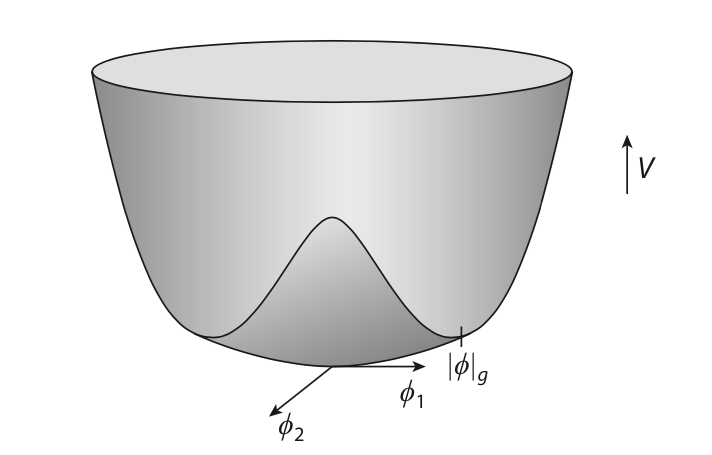
\includegraphics[width = 0.5\textwidth]{images/higgs-potential.png}
    \caption{Higgs potential from equation \eqref{eq:singlet_higgs_pot} in the complex plane (retrieved from \cite{goldberg_standard_2017}).}
    \label{fig:higgs}
\end{figure}

However, this  VEV is not unique, it is determined up to multiplication by a phase factor. This means that the Lagrangian for this scalar obeys a $U(1)$ symmetry. $SU(2)_L$ symmetry is further imposed by turning the scalar field into a doublet of the form $$\Phi = \mqty(\phi_1 \\ \phi_2),$$ called the Higgs doublet. To account for this new doublet structure, the Lagrangian from equation \eqref{eq:singlet_higgs_lag} becomes
\begin{equation}
    \mathcal{L} = \frac{1}{2}\dcov \Phi \dcon \Phi^\dagger - V(\Phi),
\end{equation}
with
\begin{equation}\label{eq:higgs_pot}
    V(\phi) = -\mu^2 \Phi\Phi^\dagger + \lambda(\Phi\Phi^\dagger)^2.
\end{equation}

As a gauge choice, let the VEV for the scalar doublet be
\begin{equation}
    \Phi_0 = \mqty (0 \\ \frac{v}{\sqrt{2}}),
\end{equation}
where $v=\mu/\sqrt{\lambda}$. The choice of the ground state spontaneously breaks the $U(1)$ symmetry of the potential, which entails the existence of two Goldstone bosons, one for each component of the doublet \cite{goldberg_standard_2017}. These Goldstone bosons can be seen when considering a small excitation of the Higgs doublet:
\begin{equation}
    \Phi =\mqty (\phi_1(x) \\ \frac{v+H(x)}{\sqrt{2}}e^{i\alpha(x)}),
\end{equation}
where $H$ and $\alpha$ are real scalar fields.
The scalar Lagrangian then expands to
\begin{equation}
    \lag = \dcov \phi_1 \dcon \phi_1^* + \frac{1}{2}\qty(v+H)^2 \dcov \alpha \dcon \alpha + \frac{1}{2}\dcov H \dcon H - \mu^2 H^2 + \text{self-interaction terms}.
\end{equation}
The $\phi_1$ Goldstone boson only interacts with itself and may be disregarded, while the $\alpha$ Goldstone boson interacts with itself and the $H$ boson. These terms are not of interest. The last two terms are however important: they represent a real scalar particle with mass $\mu = M_H$.

Returning to the $SU(2)_L\times U(1)$ symmetry, the weak hypercharge of the scalar doublet is taken as $Y_H = 1$ \cite{goldberg_standard_2017}, so it transforms under $SU(2)_L\times U(1)$ as
\begin{equation}
    \Phi \rightarrow e^{-ig'\theta^0/2}e^{-ig_W\theta_i\sigma_i/2}\Phi.
\end{equation}
As is the case for fermions, a local $SU(2)\times U(1)$ brings about interactions with gauge bosons via the covariant derivative 
\begin{equation}
    D_\mu = \dcov + i\frac{g'}{2}B_\mu + i \frac{g_W}{2} \sigma_i W^{i}_{\mu}.
\end{equation}
The Lagrangian for the scalar field becomes
\begin{equation}
    \lag_{\Phi} = D_\mu \Phi D^\mu \Phi^\dagger - V(\Phi).
\end{equation}
Ignoring the presence of Goldstone bosons, all off-diagonal terms in the kinetic part of the Lagrangian are zero. Thus, the covariant derivative introduces terms of the form
\begin{equation}
    \frac{1}{8}(v+H)^2\qty[\qty(g' B_\mu - g_W W_{\mu}^3)^2 + g_W^2(W^1)^2 + g_W^2(W^2)^2].
\end{equation}
Weinberg's rotation turns this expression into
\begin{equation}
    \lag_{\text{mass}} = \frac{1}{2} M_Z^2 Z_{\mu}Z^{\mu} + \frac{1}{2} M_W^2 W^+_{\mu} W^{-\;\mu},
\end{equation}
where
\begin{align}
    M_W &= \frac{M_H}{\sqrt{8\lambda}},\\
    M_Z &= \frac{M_W}{\cos{\theta_W}}.
\end{align}
This explains the mass of gauge bosons via the Higgs mechanism.

Fermion mass is obtained by introducing Yukawa interaction terms in the Lagrangian of the form
\begin{equation}
    -\lambda \overline{\psi} \Phi \psi.
\end{equation}
Upon splitting fermionic spinors into left- and right-handed components, allowing only terms that are gauge invariant, and relaxing the scalar doublet into the chosen ground state, these terms become
\begin{equation}
    -\lambda\frac{v}{\sqrt{2}}\overline{\psi}_L\overline{\psi}_R,
\end{equation}
which represent mass terms for the fermionic fields.

\subsubsection*{Strong interaction}
    
    
The symmetry group for the strong interaction is $SU(3)_C$, where $C$ stands for the coloured charge. Hence, the strong interaction is referred to as chromodynamics. Quarks come in three colours: red, blue and green. Thus, they are expressed as column vectors:
$$\psi = \mqty( q_r \\ q_b \\ q_g).$$
The free quark Lagrangian is
\begin{equation}
    \mathcal{L} = i \overline{\psi}_i\gamma^\mu \dcov \psi_i-m_i\overline{\psi}_i\psi_i,
\end{equation}
where the index stands for the flavour of the quark. There are six quark flavours: up, down, strange, charm, top, and bottom.

The symmetry in the Lagrangian is now incorporated. A general $SU(3)$ transformation is of the form
\begin{equation}
    \psi \rightarrow e^{-ig_s\theta_\alpha\lambda_\alpha} \psi,
\end{equation}
where $\lambda_\alpha$ are the eight generators of the $SU(3)$ Lie algebra. The corresponding Noether current is
\begin{equation}
    J^{(\alpha)\mu} = g_s \overline{\psi}\gamma^\mu\lambda_\alpha \psi.
\end{equation}
As in $SU(2)$, the gauge invariant fields transform by
\begin{equation}
    G_{\mu}^{\alpha} \rightarrow G_{\mu}^{\alpha} + \dcov \theta^\alpha - 2 \sum_{j,k} f^{\alpha jk}G_{\mu}^{j}\theta^{k},
\end{equation}
where $f^{ijk}$ are the structure constants of the $SU(3)$ Lie algebra. These fields are known as gluon fields. The covariant derivative is 
\begin{equation}
    D_\mu = \dcov +\frac{i}{2}g_s\lambda_{\alpha}G_{\mu}^{\alpha}.
\end{equation}
The Faraday tensor for gluons is
\begin{equation}
    F_{\mu\nu}^{\alpha} = D_\mu G_\nu^\alpha - D_\nu G_\mu ^\alpha = \dcov G_\nu^\alpha -\dcov[\nu] G_{\mu}^\alpha +2g_s\sum_{jk}f^{jkl}G_{\mu}^{k}G_\nu^{l}.
\end{equation}
This results in the chromodynamic Lagrangian:
\begin{equation}
    \mathcal{L}_\text{S} = \overline{\psi}(i\gamma^\mu\dcov-m)\psi-G_\mu^{\alpha}J^{(\alpha)\mu}-\frac{1}{16}F^{(k)\mu\nu}F_{(k)\mu\nu}.
\end{equation}


% The Lagrangian term
    
\subsection{Experimental Particle Physics}
Particle physics experiments often consist in detecting and identifying particles produced in high-energy collisions in particle accelerators \cite{thomson_modern_2013}. In particular, this section concerns itself with experiments carried out at CERN's Large Hadron Collider (LHC). In what follows, the Compact Muon Solenoid (CMS) experiment built at the LHC is described.

The detector has a cylindrical geometry as shown in figure \ref{fig:cms-detector}. It is $21.6\;\si{m}$ long and has a diameter of $14.6\;\si{m}$. Its total weight is $12500$ tonnes. The detector exhibits a layered design, with different subdetectors and components in each layer. The innermost layer consists of pixel detectors and silicon trackers. This layer enables the precise and efficient measurement of the trajectories of charged particles emerging from collisions. Surrounding this layer, are the electromagnetic (ECAL) and hadronic (HCAL) calorimeters. The ECAL uses lead tungstate (PbWO$_4$) crystals to efficiently absorb charged particles and transform their energy into a measurable signal. The HCAL has a similar operation. The next layer has a superconducting solenoid, which produces a large uniform magnetic field enabling the measurement of charged particle momenta. Finally, the outermost layer is the muon detector system. It has the capability of reconstructing the momentum and charge of muons \cite{CMS_experiment}.

\begin{figure}
    \centering
    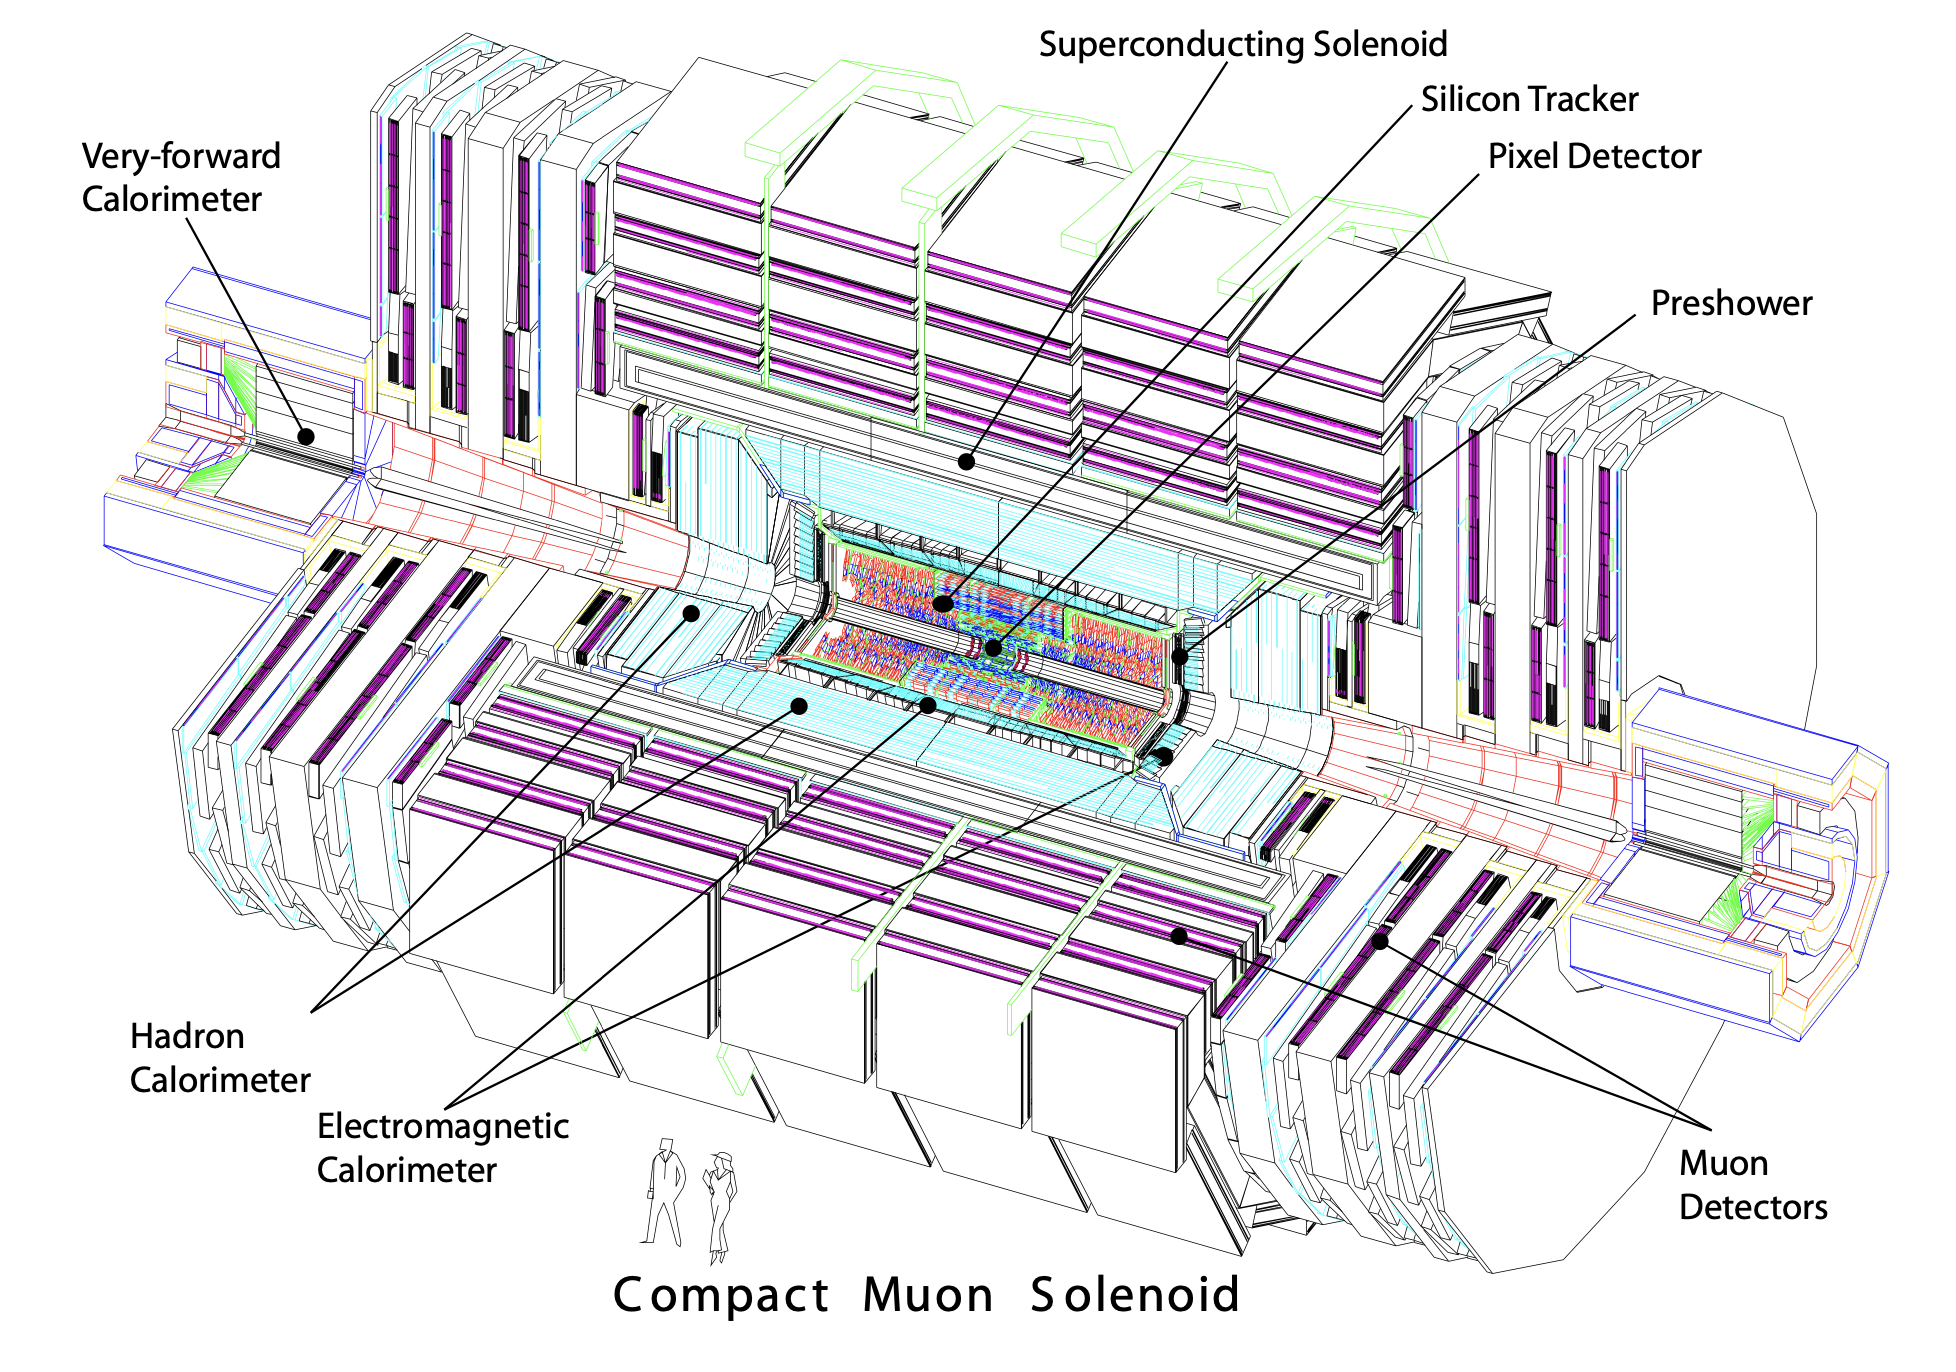
\includegraphics[width = 0.8\textwidth]{images/cms-detector.png}
    \caption{Diagram of the CMS detector showing inner components (retrieved from \cite{CMS_experiment}).}
    \label{fig:cms-detector}
\end{figure}

Measurements by the CMS adopt the coordinate system whose origin lies at the collision point, the $y$-axis pointing vertically upward, the $x$-axis pointing radially inward toward the centre of the LHC and the $z$-axis along the beam direction, towards the Jura mountains (see fig. \ref{fig:coordinate_sys}). The azimuthal angle $\phi$ is measured in the $xy$-plane from the $x$-axis and the polar angle, $\theta$, is measured from the $z$-axis.

\begin{figure}
    \centering
    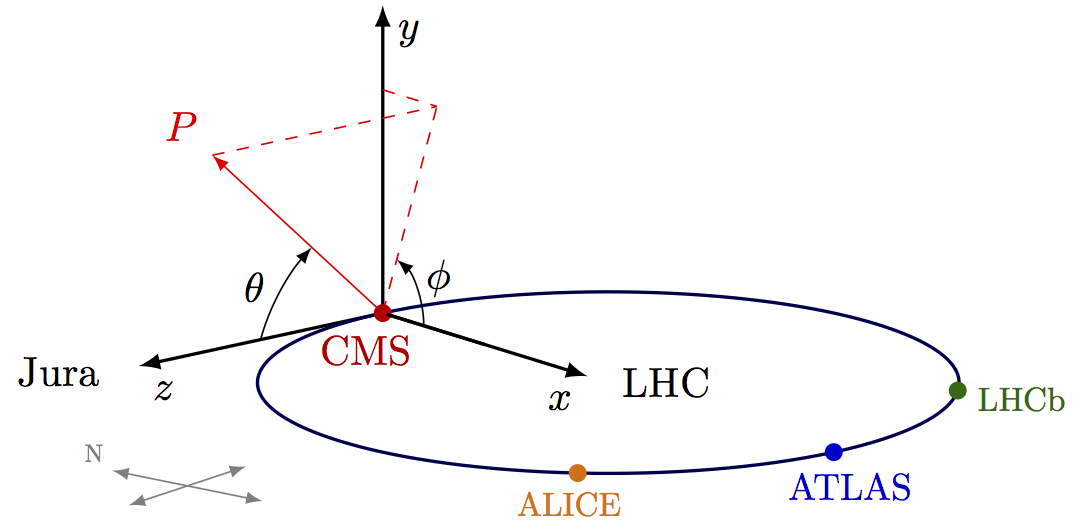
\includegraphics[width = 0.58\textwidth]{images/cms_coordinate_system.png}
    \caption{Coordinate system employed by the CMS experiment.}
    \label{fig:coordinate_sys}
\end{figure}

\subsubsection*{Experimental variables}
A key element of any experiment is the set of variables that will be measured. Thus, in order to fully describe the CMS experiment, some of its parameters should be outlined. The two most important parameters of an accelerator are the following:
\begin{description}
    \item[Luminosity ($\mathcal{L}$)] Measures the ability of an accelerator to generate interactions; it establishes a proportionality between the rate of interactions, $dR/dt$, and the production cross-section, $\sigma$ (defined below).
    \begin{equation}
        \dv{R}{t} = \mathcal{L} \sigma.
    \end{equation}
    For LHC beams, which collide head-on with a gaussian density distribution and come in bunches, the luminosity is given by $$\mathcal{L} = \frac{f N_1 N_2 N_b}{4\pi \sigma_x \sigma_y},$$ where $N_1$, $N_2$ are the numbers of particles in each colliding bunch, $f$ is the frequency at which bunches collide, $N_b$ is the number of bunches, and $\sigma_{x}$, $\sigma_{y}$ are the density deviations along the $x$ and $y$-axes, respectively \cite{herr-luminosity,thomson_modern_2013}.
    
    The luminosity can be integrated in time to obtain a direct relationship between event number and the cross-section:
    \begin{align}
        L = \int \mathcal{L}\, dt,\\
        N = L\sigma.
    \end{align}
    
    \item[Centre-of-mass energy ($\sqrt{s}$)] The energy of the colliding particles in the centre-of-mass (CM) frame. Since the total momentum of the particles in the CM frame is zero, the CM energy is simply the square-root of the total 4-momentum:
    \begin{align}
        \sqrt{s} = \sqrt{P^\mu P_\mu},\\
        P^\mu = \sum_{i} p^{\mu}_{i}.
    \end{align}
    The energy in the CM frame must be greater than the total mass of the particles being produced. Thus, the CM energy determines which particles can be studied in the accelerator.
    
\end{description}

The following variables are related to the particles being produced rather than the accelerator.
\begin{description}
    \item[Decay width ($\Gamma$)] The decay rate is the probability that a given particle will decay per unit time. Since a particle can suffer multiple decay modes, the total decay rate is the sum of the decay rates for each mode \cite{thomson_modern_2013}. The relative frequency of a decay mode is the \textit{branching ratio}, given by
    \begin{equation}
        \operatorname{BR}(j) = \frac{\Gamma(j)}{\Gamma}.
    \end{equation}
    
    \item[Cross-section ($\sigma$)] The cross-section is a measure of the probability that an interaction will occur from a collision. It is a quantum-mechanical analogue of the ``effective size'' of the particles involved in an interaction. It is related to the decay width according to
    \begin{equation}
        \Gamma = \rho\sigma v,
    \end{equation}
    where $\rho$ is the number density of particles and $v$ is the relative velocity of the incoming particles \cite{thomson_modern_2013}.
    
    \item[Pseudo-rapidity ($\eta$)] Instead of using the polar angle, CMS measurements involve the pseudo-rapidity, defined by
    \begin{equation}
        \eta = - \ln(\tan{\frac{\theta}{2}}).
    \end{equation}
    The main advantage of using the pseudo-rapidity is that distributions over it tend to be closer to a uniform distribution than those over the polar angle. Furthermore, the difference in pseudo-rapidity is invariant under Lorentz boosts along the beam direction \cite{thomson_modern_2013}.
    
    \item[Missing transverse energy and momentum ($E^{\mathrm{miss}}_T$ \& $p^{\mathrm{miss}}_T$)]
    Missing energy and momentum refers to the energy and momentum that is not detected but is expected to be there as a consequence of energy and momentum conservation. This momentum is often carried by particles that do not interact electromagnetically or strongly and are therefore difficult to detect \cite{thomson_modern_2013}. Missing energy and momentum provide an indirect measurement of undetectable particles in hadron colliders such as neutrinos. Missing momentum reconstructions focus on the transverse direction, where total momentum is expected to be zero.
    
\end{description}


\section{State of the Art}

Leptoquarks (LQs) are hypothetical particles that can decay into a quark and a lepton. They introduce vertices like the one shown in figure \ref{fig:vertex}. Such particles often arise in Grand Unified Theories (GUTs) such as the Pati-Salam model \cite{pati_lepton_1974, baker_high_2019} and GUTs based on $SU(5)$, $SO(10)$, and larger gauge groups \cite{goldberg_standard_2017, da_rold_vector_2019}. 

\begin{figure}[b]
    \centering
    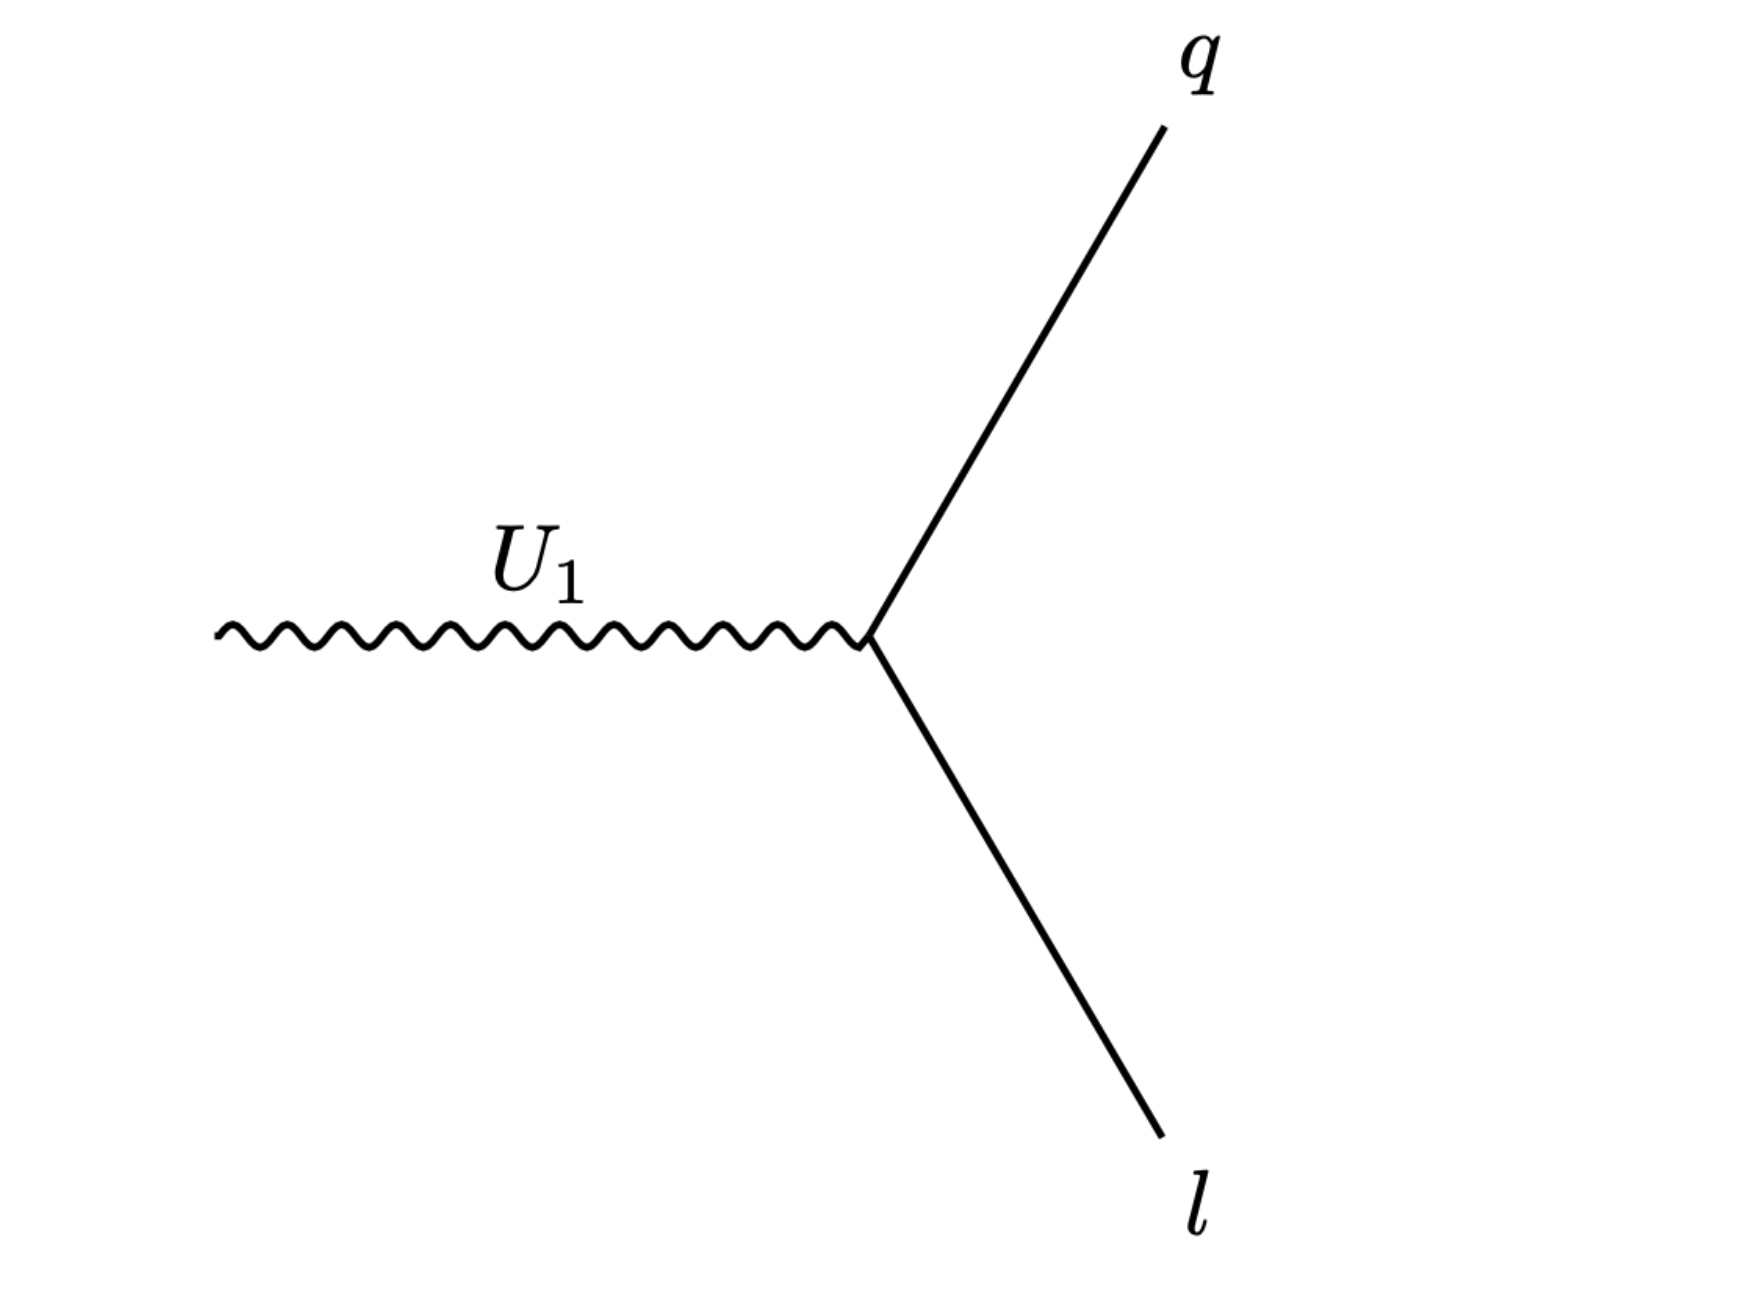
\includegraphics[width = 0.3\textwidth]{images/lq-vertex.png}
    \caption{Feynman diagram vertex showing a LQ coupling to a quark $q$ and a lepton $l$.}
    \label{fig:vertex}
\end{figure}

A consequence of the introduction of LQs is the non-conservation of baryon and lepton number, which are accidentally conserved quantities within the SM. This is the extent to which the manifold of models that predict LQs agree. To exemplify the diversity of LQs one can find in the literature, as summarised in \cite{zyla_review_2020}, table \ref{tab:quantum_num} is compiled. Since the interactions between LQs and SM fermions are assumed to be invariant under the SM symmetry group ($G_{\text{SM}}$), the $G_{\text{SM}}$ quantum numbers of possible LQs can distinguish different ``types'' of LQ. Table \ref{tab:quantum_num} shows possible quantum numbers for LQs and their allowed interactions. Notice that LQ spin is either 0 (scalar) or 1 (vector). 

\begin{table}
    \centering
    \begin{tabular}{c c c c c }
        \toprule
        Spin & $SU(3)_c$ & $SU(2)_L$ & $U(1)_Y$ & Allowed coupling \\ \midrule
        0 & $\overline{3}$ & 1 & 1/3 & $\overline{q}^{c}_{L} \ell_L $ or $\overline{u}_{R}^c e_R$ \\
        0 & $\overline{3}$ & 1 & 4/3 &  $\overline{d}_{R}^c e_R$ \\
        0 & $\overline{3}$ & 3 & 1/3 &  $\overline{q}_{L}^c \ell_L$ \\
        0 & 3 & 2 & 7/6 & $\overline{q}_{L} e_R $ or $\overline{u}_{R} \ell_L$ \\
        0 & 3 & 2 & 1/6 & $\overline{d}_{R} \ell_L$ \\
        1 & $\overline{3}$ & 2 & 5/6 &  $\overline{q}^{c}_{L} \gamma^\mu e_R $ or $\overline{d}_{R}^c \gamma^\mu \ell_L$ \\
        1 & $\overline{3}$ & 2 & -1/6 &  $\overline{u}_{R}^c \gamma^\mu \ell_L$ \\
        1 & 3 & 1 & 2/3 &  $\overline{q}_{L} \gamma^\mu \ell_L$ or $\overline{d}_{R} \gamma^\mu e_R$ \\
        1 & 3 & 1 & 5/3 &  $\overline{u}_{R} \gamma^\mu e_R$ \\
        1 & 3 & 3 & 2/3 &  $\overline{q}_{L} \gamma^\mu \ell_L$ \\
        \bottomrule
    \end{tabular}
    \caption{Elementary Particles of the Standard Model (the number at the end of each row of fermions is the generation number)}
    \label{tab:quantum_num}
\end{table}


Models that include LQs with masses in the TeV scale have become of interest for explaining $B$-meson decay anomalies, since they allow for non-universal coupling strengths to leptons \cite{di_luzio_gauge_2017}. According to \cite{baker_high_2019}, the minimal gauge group containing a vector leptoquark that explains the anomalies and is consistent with high transverse momentum ($p_T$) data is $$G_{4321} = SU(4) \times SU(3)' \times SU(2)_L \times U(1)'.$$ This gauge group can be regarded as a low-energy limit of the $PS^3$ model proposed in \cite{bordone_three-site_2018} and furthermore it can accommodate spontaneous symmetry breaking to produce masses for three new gauge bosons: a vector LQ ($U_1$), a neutral boson ($Z'$) and a coloron ($G'$) \cite{cornella_revisiting_2019}.
 
$$
\begin{aligned}
\mathcal{L}_{U_{1}}=&-\frac{1}{2} U_{1 \mu \nu}^{\dagger} U_{1}^{\mu v}+M_{U}^{2} U_{1 \mu}^{\dagger} U_{1}^{\mu} \\
&-i g_{s}\left(1-\kappa_{U}\right) U_{1 \mu}^{\dagger} T^{a} U_{1 v} G^{a \mu v} \\
&-i g_{Y} \frac{2}{3}\left(1-\tilde{\kappa}_{U}\right) U_{1 \mu}^{\dagger} U_{1 v} B^{\mu v} \\
&+\frac{g_{U}}{\sqrt{2}}\left[U_{1}^{\mu}\left(\beta_{L}^{i j} \bar{q}_{L}^{i} \gamma_{\mu} \ell_{L}^{j}+\beta_{R}^{i j} \bar{d}_{R}^{i} \gamma_{\mu} e_{R}^{j}\right)+\text { h.c. }\right]
\end{aligned}
$$





